\documentclass[11pt, openright]{book}

	% Cover Variables
	\newcommand{\ctitle}{DC MOTORS}
	\newcommand{\cautor}{Lucas Lescure - Eva Maturana}
	\newcommand{\ctoptitle}{REPORT TP ENER}

	% Header Variables
		\newcommand{\headRE}{\emph{\thepage}}
		\newcommand{\headLE}{\emph{\thesection. \rightmark}}
		\newcommand{\footRE}{}
		\newcommand{\footLE}{}

	% TOC Variables
		\newcommand{\toctitle}{Table of Content}
		\newcommand{\tocchapter}{Chapter}
		\newcommand{\toccount}{3}
  
	% Chapter Variables
		\newcommand{\chvar}{Chapter -}

\usepackage[a4paper, total={16cm, 22.125cm}]{geometry}

% Page Style
\usepackage[]{environ}
% Cover Page 
\usepackage{tikz}
\makeatletter
\def\parsecomma#1,#2\endparsecomma{\def\page@x{#1}\def\page@y{#2}}
\tikzdeclarecoordinatesystem{page}{
    \parsecomma#1\endparsecomma
    \pgfpointanchor{current page}{north east}
    % Save the upper right corner
    \pgf@xc=\pgf@x%
    \pgf@yc=\pgf@y%
    % save the lower left corner
    \pgfpointanchor{current page}{south west}
    \pgf@xb=\pgf@x%
    \pgf@yb=\pgf@y%
    % Transform to the correct placement
    \pgfmathparse{(\pgf@xc-\pgf@xb)/2.*\page@x+(\pgf@xc+\pgf@xb)/2.}
    \expandafter\pgf@x\expandafter=\pgfmathresult pt
    \pgfmathparse{(\pgf@yc-\pgf@yb)/2.*\page@y+(\pgf@yc+\pgf@yb)/2.}
    \expandafter\pgf@y\expandafter=\pgfmathresult pt
}
\makeatother


% Object formatting
\usepackage[12pt]{moresize}
\usepackage[]{anyfontsize}
\usepackage{titlesec}
\usepackage{import}
\usepackage{floatrow}
\usepackage{enumitem}
\usepackage{changepage}
\usepackage[normalem]{ulem}
\usepackage{array}
\newcommand{\ul}[1]{\underline{#1}}

\usepackage[]{chngcntr}
\usepackage{ifthen}
\ifthenelse{\figcountdepth > 1}
  {\counterwithin{figure}{section}\counterwithin{table}{section}}
  {}

\usepackage[format=plain, labelfont=it, textfont=it]{caption}
\makeatletter
\def\@makecaption#1#2{%
    \vskip\abovecaptionskip
    \sbox\@tempboxa{\textit{#1.} #2}

       
   

    \ifdim \wd\@tempboxa >\hsize
        #1. #2\par
    \else
        \global \@minipagefalse
        \hb@xt@\hsize{\hfil\box\@tempboxa\hfil}
    \fi
    \vskip\belowcaptionskip}
\makeatother

\DeclareCaptionFormat{underline}{\uline{#1#2#3}\par}

% Sections
\titleformat{\section}{\fontsize{16}{19.2}\bfseries}{\thesection.}{0.25em}{}
\titleformat{\subsection}{\fontsize{14}{16.8}\bfseries}{\tab\thesubsection.}{0.25em}{}
\titleformat{\subsubsection}{\fontsize{10}{12}}{\uline{\thesubsubsection)\enspace}}{0em}{\uline}





% Geometry

% Typewritting

\setlength{\parskip}{1em}
\setlength{\parindent}{0em}


\newenvironment{items}[3][0pt]
{\def\closesep{#3}
    \vspace{#2}
    \begin{itemize}
        \setlength{\itemsep}{#1}
        \setlength{\topsep}{0pt}
        \setlength{\partopsep}{0pt}}
        {\end{itemize}
    \vspace{\closesep}}

\newenvironment{enum}[3][0pt]
{\defclosesep{#3}
    \vspace{#2}
    \begin{enumerate}
        \setlength{\itemsep}{#1}
        \setlength{\topsep}{0pt}
        \setlength{\partopsep}{0pt}}
        {\end{enumerate}
    \vspace{\closesep}}

\newenvironment{eq}[2]
{\def\closesep{#2}
    \vspace{#1}
    \begin{align*}}
        {\end{align*}
    \vspace{\closesep}}

\newenvironment{lfeq}[2]
{\def\closesep{#2}
    \vspace{#1}
    \begin{flalign*}}
        {\end{flalign*}
    \vspace{\closesep}}
% List Formatting


\NewEnviron{dent}[1]{
    \vspace{-10pt}
    \begin{adjustwidth}{7mm}{}
        \uline{#1}\hspace{2mm}
        \BODY
    \end{adjustwidth}
    \vspace{-10pt}
}


\usepackage[framemethod=tikz]{mdframed}
\newcounter{count_theorem}[section]\setcounter{count_theorem}{0}
\newcommand{\thetheorem}{\arabic{count_theorem}}

\newcounter{count_exercise}[section]\setcounter{count_exercise}{0}
\newcommand{\theexercise}{\arabic{count_exercise}}


\newenvironment{theorem}[1][]{
    \refstepcounter{count_theorem}
    \mdfsetup{
        linecolor=red!30,
        innerbottommargin=10pt,
        linewidth=2pt,
        topline=false,
        bottomline=false,
        rightline=false,
        shadow=true,
        shadowsize=4.5pt,
        frametitlerule=false,
        apptotikzsetting={
                \tikzset{
                    mdfbackground/.append style={
                            left color=red!8,right color=red!3
                        }
                }
            }
    }
    \begin{mdframed}[]\relax
        \ifstrempty{#1}
        {\textbf{Theorem~\thetheorem.} }
        {\textbf{Theorem~\thetheorem.~#1} }
        }
        {\end{mdframed}\vspace{-10pt}
}

\newenvironment{note}{
    \mdfsetup{innertopmargin=5pt,
        linecolor=gray!30,
        linewidth=2pt,
        topline=false,
        bottomline=false,
        rightline=false,
        frametitleaboveskip=0pt,
        shadow=false,
        shadowsize=4pt,
        frametitlerule=false,
        apptotikzsetting={
                \tikzset{
                    mdfbackground/.append style={
                            left color=gray!8,right color=gray!3
                        }
                }
            }
    }
    \begin{mdframed}[]\relax
        \textbf{Note. }
        }
        {\end{mdframed}\vspace{-10pt}
}

\newenvironment{example}{
    \mdfsetup{innertopmargin=5pt,
        linecolor=green!30,
        linewidth=2pt,
        topline=false,
        bottomline=false,
        rightline=false,
        frametitleaboveskip=0pt,
        shadow=false,
        shadowsize=4pt,
        frametitlerule=false,
        apptotikzsetting={
                \tikzset{
                    mdfbackground/.append style={
                            left color=green!7,right color=green!2
                        },
                    mdfframetitlebackground/.append style={
                            left color=green!7,right color=green!2
                        }
                }
            }
    }
    \begin{mdframed}[]\relax
        \textbf{Example. }
        }
        {\end{mdframed}\vspace{-10pt}
}


\usetikzlibrary{calc,arrows}

\tikzset{
    excursus arrow/.style={%
            line width=2pt,
            draw=gray!40,
            rounded corners=2ex,
        },
    excursus head/.style={
            fill=white,
            font=\bfseries\sffamily,
            text=gray!80,
            anchor=base west,
        },
    excursus line/.style={%
            line width=2pt,
            draw=gray!40,
            rounded corners=2ex,
        }
}

\newenvironment{exercise}[1][]{%
    \refstepcounter{count_exercise}
    \mdfsetup{
        singleextra={
                \path let \p1=(P), \p2=(O) in (\x2,\y1) coordinate (Q);
                \path let \p1=(Q), \p2=(O) in (\x1,{(\y1-\y2)/2}) coordinate (M);
                \path [excursus line] ($(O)+(5em,0ex)$) -| (M) |- ($(Q)+(20em,0ex)$);
                \node [excursus head] at ($(Q)+(2.5em,-0.75pt)$) {\ifstrempty{#1}{Exercise \theexercise}{Exercise \theexercise:~#1}};},
        firstextra={
                \path let \p1=(P), \p2=(O) in (\x2,\y1) coordinate (Q);
                \path [excursus arrow,-to] (O) |- ($(Q)+(12em,0ex)$) .. controls +(0:16em) and +(185:6em) .. ++(23em,2ex);},
        middlelinewidth=2.5em,middlelinecolor=white,
        hidealllines=true,topline=true,
        innertopmargin=0.5ex,
        innerbottommargin=2.5ex,
        innerrightmargin=2pt,
        innerleftmargin=2ex,
        skipabove=0.87\baselineskip,
        skipbelow=0.62\baselineskip,
    }
    \begin{mdframed}[]\relax}
        {\end{mdframed}\vspace{-10pt}
}

% Functions and Data Plotting
\usepackage{subfig,wrapfig,adjustbox,multirow}


% Plotting Style
\usepackage{graphicx,pgfplots}
\usetikzlibrary{arrows}
\usetikzlibrary {patterns,patterns.meta}
\usepgfplotslibrary{fillbetween}
\pgfplotsset{compat=1.18}

\usepgfplotslibrary{units}
% Logarithmic Scale
\pgfplotsset{
    log x ticks with fixed point/.style={
            xticklabel={
                    \pgfkeys{/pgf/fpu=true}
                    \pgfmathparse{exp(\tick)}%
                    \pgfmathprintnumber[fixed relative, precision=3]{\pgfmathresult}
                    \pgfkeys{/pgf/fpu=false}
                }
        }
}


% Mathematics

% Formatting
\usepackage{amsmath}
\usepackage{esvect}
\usepackage{amsfonts}
\usepackage{tasks,environ}
\usepackage{xargs}
\usepackage{esint}
\usepackage[]{listings}


\usepackage[english]{babel}
\usepackage{amsthm}
%\newtheorem{theorem}{Theorem}
%\newtheorem{proof}{Proof}



%Custom Shortcuts
\newcommand{\eqi}{\Leftrightarrow}
\newcommand{\lr}[1]{\left( #1 \right)}
\newcommand{\limit}[1]{\displaystyle{\lim_{#1}}}
\newcommand{\tab}{\hspace*{7mm}}
\newcommand{\ds}[1]{\displaystyle{#1}}
\newcommand{\floor}[1]{\lfloor #1 \rfloor}
\newcommand{\R}{\mathbb{R}}
\newcommand{\N}{\mathbb{N}}
\newcommand{\Z}{\mathbb{Z}}
\newcommand{\C}{\mathbb{C}}
\newcommand{\K}{\mathbb{K}}
\newcommand{\F}{\mathcal{F}}
\newcommand{\M}{\mathcal{M}}
\renewcommand{\l}{\lambda}
\newcommand{\seg}[1]{\overline{\rm {#1}}}
\newcommand{\Int}{\int\limits}
\newcommand{\ex}{\tab \uline{Example :}\hspace{0.2cm} }
\newcommand{\vard}{\partial}
\newcommand{\Q}{\mathcal{Q}}
\newcommand{\Vect}{\operatorname{Vect}}
\newcommand{\rg}{\operatorname{rg}}
\renewcommand{\dim}{\operatorname{dim}}
\renewcommand{\Re}{\operatorname{Re}}
\renewcommand{\Im}{\operatorname{Im}}
\renewcommand{\P}{\mathcal{P}}
\newcommand{\blr}[1]{\left\{#1\right\}}
\newcommand{\linecenter}[1]{\par\vspace{2mm} \centerline{#1}\par\vspace{-2mm}}
\newcommand{\dd}{\textrm{d}}
\newcommand{\supp}{\operatorname{Supp}}
\renewcommand{\vec}{\overrightarrow}
\renewcommand{\epsilon}{\varepsilon}

% Matrix Configurations

\makeatletter
\renewcommand*\env@matrix[1][*\c@MaxMatrixCols c]{%
    \hskip -\arraycolsep
    \let\@ifnextchar\new@ifnextchar
    \array{#1}}
\makeatother


% Colors
\usepackage{xcolor}
\newcommand{\blu}{\color{blue}}
\newcommand{\Red}{\color{red}}
\newcommand{\blac}{\color{black}}

\newcommand{\red}[1]{\textcolor{red}{#1}}

\usepackage{xcolor,xspace}
\usepackage{breqn}


% Headings  
\usepackage[Glenn]{fncychap}
\ChNumVar{\fontsize{40}{42}}
\ChTitleVar{\Large\sc}
\ChNameVar{\Large\sc}
\setlength\headheight{14.5pt}
\renewcommand\FmN[1]{\chvar}



\usepackage{fancyhdr}
\usepackage{ragged2e}

% Header & Footers
\renewcommand{\chaptermark}[1]{\markboth{#1}{#1}}
\renewcommand{\sectionmark}[1]{
    \markright{ #1}
}
\pagestyle{fancy}
\fancyhf{}
\fancyhead[LE,RO]{\headLE}
\fancyhead[RE,LO]{\headRE}
\fancyfoot[LE,RO]{\footLE}
\fancyfoot[RE,LO]{\footRE}
\renewcommand{\headrulewidth}{0.5pt}
\fancyheadoffset{1cm}

\fancypagestyle{plain}{%
    \fancyhf{} % clear all header and footer fields
    \fancyfoot[LE, RO]{\footLE}
    \renewcommand{\headrulewidth}{0pt}
    \renewcommand{\footrulewidth}{0pt}}


\fancypagestyle{nohead}{%
    \fancyhf{} % clear all header 
    \fancyfoot[LE, RO]{\footLE}
    \fancyfoot[LO, RE]{\footRE}}

    \fancypagestyle{head}{%
    \fancyhf{} % clear all header 
    \fancyhead[LE,RO]{\headLE}
\fancyhead[RE,LO]{\headRE}
\renewcommand{\headrulewidth}{0.5pt}
\fancyheadoffset{1cm}
    }


\fancypagestyle{bib}{%
    \fancyhf{} % clear all header and footer fields
    \fancyhead[CE, CO]{}
    \fancyfoot[LE, RO]{\footLE}
    \fancyfoot[LO, RE]{Bibliographie}}

% Table of Contents

\renewcommand*\thechapter{\arabic{chapter}} %Usually Roman
\renewcommand*\thesection{\arabic{section}}
\renewcommand*\thesubsubsection{\thesubsection.\alph{subsubsection}}
\makeatletter
\@removefromreset{section}{chapter}
\makeatother


% Table of Contents

\usepackage{titletoc}
\usepackage{ erewhon,cabin}
\usepackage[linktoc=all]{hyperref}
\renewcommand*\contentsname{\centerline{\toctitle}}

\setcounter{secnumdepth}{3}
\setcounter{tocdepth}{\toccount}

\usepackage[subfigure]{tocloft}
\setlength\cftparskip{0pt}

\usepackage{etoolbox}
\makeatletter
\pretocmd{\chapter}{\addtocontents{toc}{\protect\addvspace{5\p@}}}{}{}
\pretocmd{\section}{\addtocontents{toc}{\protect\addvspace{-10\p@}}}{}{}
\pretocmd{\subsection}{\addtocontents{toc}{\protect\addvspace{1\p@}}}{}{}
\makeatother


% Chapter Style
\titlecontents{chapter}
[11em]
{\bigskip}
{\bfseries\textsc\tocchapter~\textsc\thecontentslabel : \textsc}
{\hspace*{-5.5em}\textbf}
{\titlerule*[1pc]{ }}[\smallskip]

% Section Style
\titlecontents{section}
[0em] % i
{\bigskip\bfseries}
{\fontsize{11}{13.2}\bfseries\uline{\thecontentslabel.\enspace}\uline}
{\hspace*{-4em}\textbf}
{\hspace{0.5pt}\uline{\hspace*{\fill}}\contentspage}

% Subsection Style
\titlecontents{subsection}
[2em] % i
{\smallskip\bfseries}
{\fontsize{10}{12}\bfseries\thecontentslabel.\enspace}
{\hspace*{-4em}}
{\titlerule*[0.5pc]{.}\contentspage}

% Subsubsection Style
\titlecontents{subsubsection}
[4em] % i
{\smallskip}
{\fontsize{10}{12}\thecontentslabel)\enspace}
{\hspace*{-4em}}
{\titlerule*[0.5pc]{.}\contentspage}










	% figure support
	\usepackage{import}
	\usepackage{xifthen}
	\pdfminorversion=7
	\usepackage{pdfpages}
	\usepackage{transparent}
	\newcommand{\incfig}[1]{%
			\def\svgwidth{\columnwidth}
			\import{./figures/}{#1.pdf_tex}
	}

	\pdfsuppresswarningpagegroup=1

	\usepackage[american]{circuitikz} 
\usetikzlibrary{decorations.pathreplacing,calligraphy}


\begin{document}
% Spacing
% Section Spacing
\titlespacing\section{0pt}{3pt plus 2pt minus 2pt}{6pt plus 2pt minus 1pt}
\titlespacing\subsection{0pt}{0pt plus 1pt minus 1pt}{0pt plus 3pt minus 1pt}
\titlespacing\subsubsection{0pt}{0pt plus 0pt minus 0pt}{0pt plus 2pt minus 0pt}

\usetikzlibrary{shadows}

\newgeometry{left=2.5cm, width=16cm, bottom=2.5cm, top=2.5cm}






% Cover
% Cover
\definecolor{ccolor1}{RGB}{236,145,143}
\definecolor{ccolor2}{RGB}{131,168,192}
\definecolor{ccolor3}{RGB}{182,227,150}
\definecolor{ccolor4}{RGB}{171,206,145}

\usetikzlibrary{fadings}

\begin{titlepage}
    \newgeometry{top=1cm, width=21cm, bottom=1cm}

    \begin{tikzpicture}[remember picture,overlay,every node/.style={anchor=center}]

        \coordinate (Center) at (page cs: 0,-0.5);
        %F4E Logo
        \begin{scope}[scale = 1.5]
            \foreach \angle in {0,30,...,330} {
                    \filldraw[orange!50!yellow,line width=0.01pt,shift=(Center)] (\angle:3.8637) -- (\angle+30:3.8637) -- (0,0) -- (\angle:3.8637);
                    \draw[white, line width = 7pt,shift=(Center)] (\angle:2cm) arc (\angle-60:\angle:2cm);
                    \draw[white, line width = 7pt,shift=(Center)] (\angle+30:2cm) arc (\angle+90:\angle+30:2cm);
                }
            % Outer delimiter
            \foreach \angle in {15,45,...,345} {
                    \filldraw[white, line width = 7pt,shift=(Center)] (\angle:3.8637cm) arc (\angle-15:\angle+45:2cm) arc (\angle+15:\angle-15:2cm) arc (\angle+45:\angle+15:2cm);
                }
            % Inner delimiter
            \foreach \angle in {15,45,...,345} {
                    \filldraw[white, line width = 7pt,shift=(Center)] (\angle:1.0353cm) arc (\angle-75:\angle-45:2cm) arc (\angle+75:\angle+105:2cm) -- (0,0) -- (\angle:1.0353cm);
                }
            % Stars
            \foreach \angle in {0,30,...,330} {
                    \fill[orange!50!yellow,shift=(Center)] (\angle:1.03527cm) -- ++ (231:0.175) -- ++ (33:0.35) -- ++ (177:0.35) -- ++ (321:0.35) -- ++ (105:0.35) -- ++ (249:0.35) -- ++ (33:0.35);
                }
        \end{scope}

        \node[opacity =0.07, inner sep=0pt, anchor=east] at (current page.east){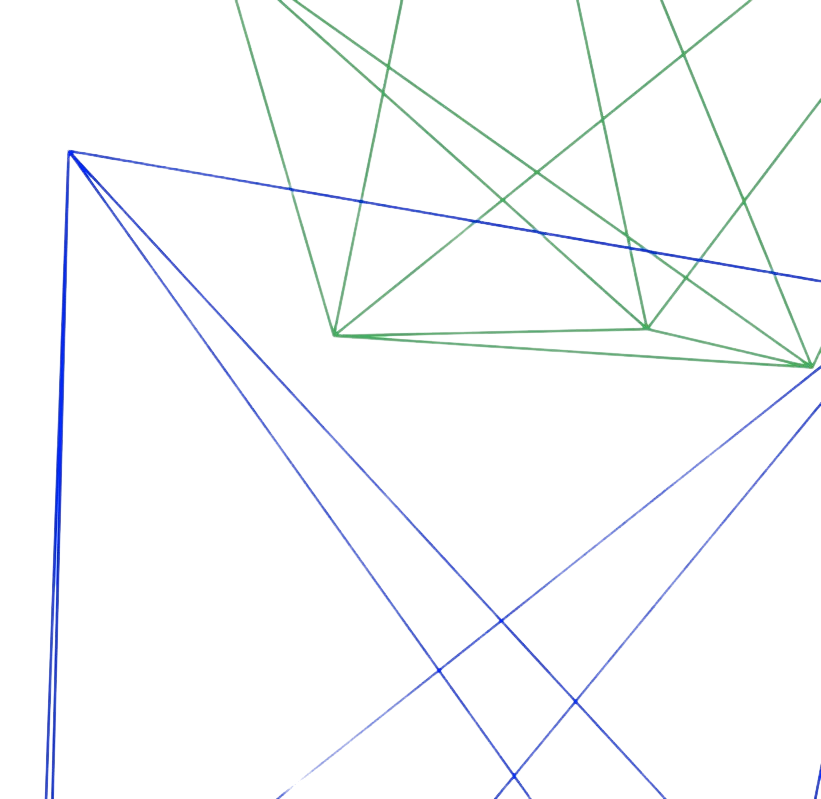
\includegraphics[width=0.5\paperwidth,height=\paperheight]{/root/.config/latex-utils/logos/invert1.png}};

        \node[opacity=0.07,inner sep=0pt, anchor=north west] at (current page.north west){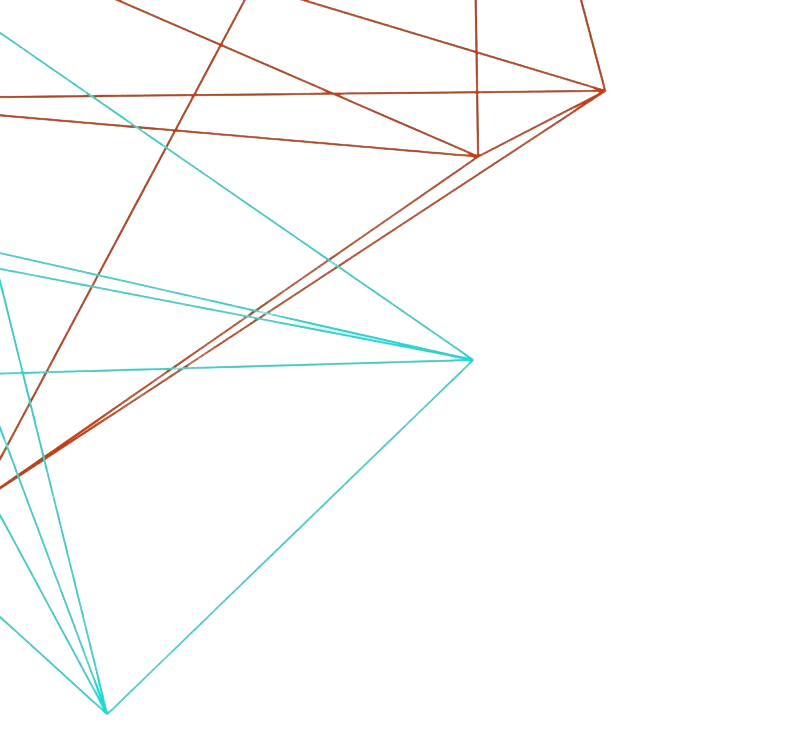
\includegraphics[width=0.5\paperwidth,height=0.5\paperheight]{/root/.config/latex-utils/logos/invert3.png}};




        \node at (page cs:0,0.345) {\Large\textsc{High School Observation and Learning Internship}};
        \node at (page cs:0,0.875) {\Large\bfseries\textsc{Observation Internship}};
        \node at (page cs:0,0.925) {\LARGE\bfseries\textsc{Lycée Français de Barcelone}};

        \node at (page cs:0.5,0) {\Large\textsc{Cyril Lescure - Pedagogical Tutor}};








        %\node[opacity=0.15, inner sep=0pt, anchor=south west] at (current page.south west){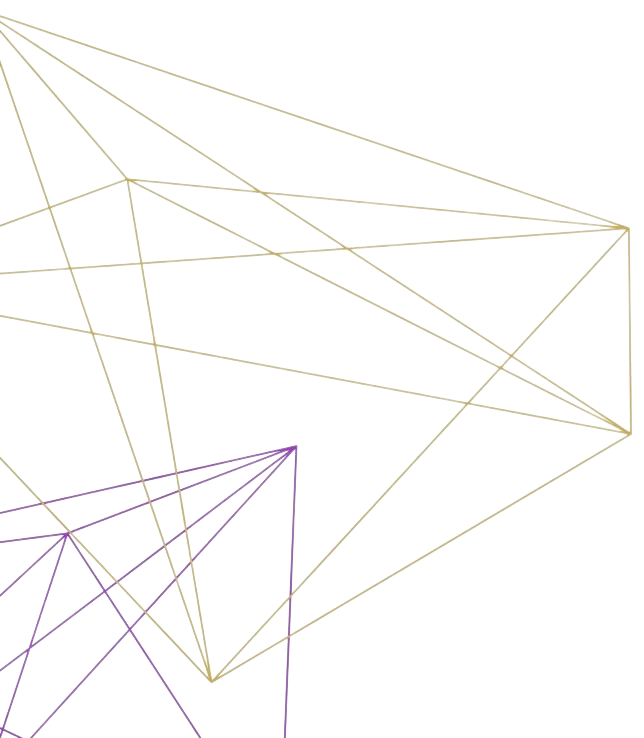
\includegraphics[width=0.5\paperwidth,height=0.5\paperheight]{/root/.config/latex-utils/logos/invert2.png}};

        \node at (page cs:0,0.5) {\fontsize{28}{28.8}\textbf{\ctoptitle}};
        \node at (page cs:0,0.425) {\fontsize{28}{28.8}\textbf{\ctitle}};
        \draw (page cs:0.5,0.375) -- (page cs:-0.5,0.375);
        \node at (page cs:0,0.245) {\LARGE\textsc{\cautor}};
        \node at (page cs:0,0.310) {\Large\textsc{03.06.2019 - 07.06.2019}};


    \end{tikzpicture}
\end{titlepage}


\newgeometry{width=18.625cm, bottom=2cm, top=2cm}

\tikz[remember picture, overlay] \node[opacity=0.3,inner sep=0pt, anchor=north east] at (current page.north east){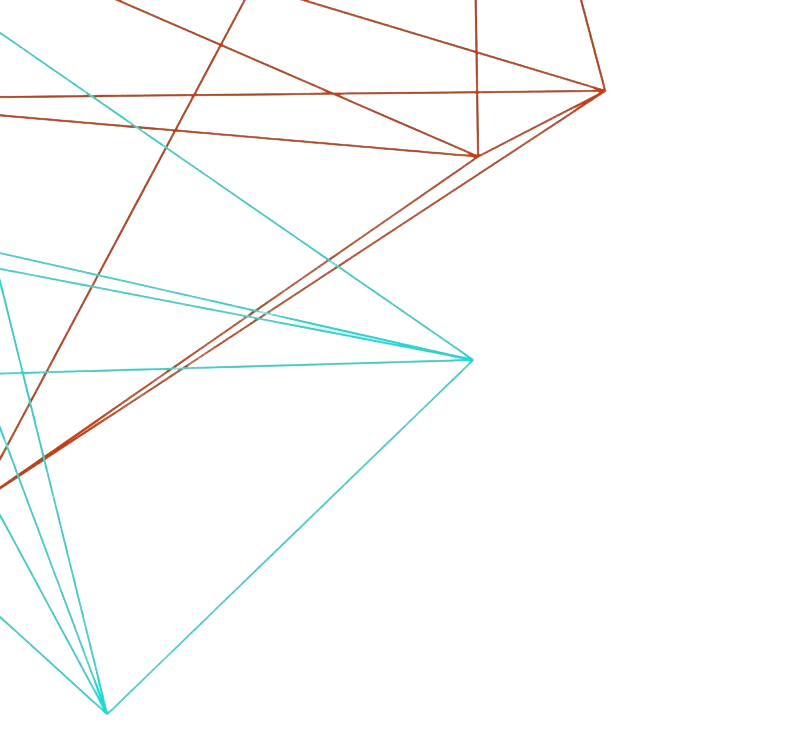
\includegraphics[angle=-90,origin=c,width=0.5\paperheight,height=0.5\paperwidth]{/root/.config/latex-utils/logos/invert3.png}};
\tikz[remember picture,overlay] \node[opacity=0.3,inner sep=0pt, anchor=south east] at (current page.south east){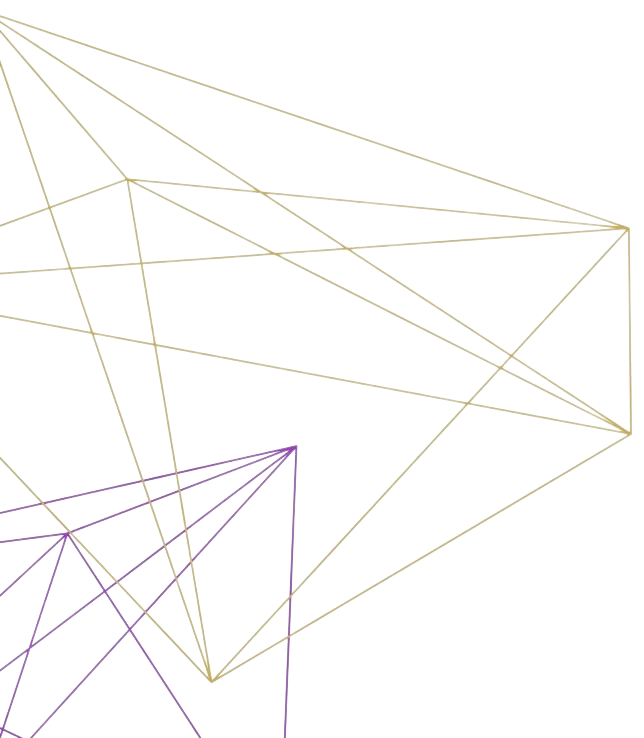
\includegraphics[angle=90,width=0.5\paperwidth,height=0.5\paperheight]{/root/.config/latex-utils/logos/invert2.png}};

\tableofcontents






\vspace*{\fill}

\section{Abstract}

We'll be studying DC Motors both in a configuration with and without a load in an attempt to better understand the principles that tie the theory translated by formulas to their direct implication in a laboratory setting. 

\newpage

\section{No-Load Experiment}

\begin{figure}[ht]
	\begin{tikzpicture}

		\node (rect) at (0,0) [draw,thick,minimum width=6cm,minimum height=3cm] {\Large DC Converter};
		\draw[very thick, black] (-2.5,0) circle (4pt); 
		\draw[very thick, black] (-2.5,0.75) circle (4pt); 
		\draw[very thick, black] (-2.5,-0.75) circle (4pt); 
		
		\draw[very thick, black] (-2.63,0) -- (-4,0);
		\draw[very thick, black] (-2.63,0.75) -- (-4,0.75);
		\draw[very thick, black] (-2.63,-0.75) -- (-4,-0.75);
		
		\draw[very thick, decorate, decoration = {calligraphic brace, amplitude=7.5pt}] (-4.25,-1) --  (-4.25,1);
		\node (rect) at (-6.1,0) [draw, thick, minimum width=3cm, minimum height=2cm, align=center] {\Large Variable AC\\ \Large Supply};
		
		\draw[thick] (2.5,1) to [battery1] (2.5,-1);
		\draw[thick] (2.5,1) -- (2.5,2) -- (6,2) -- (6,1.5);
		
		\draw[thick] (5.8,1.25) -- (5.8,1.5) -- (6.2,1.5) -- (6.2,1.25);
		\filldraw[thick, fill=white] (6,0) circle (1.25cm) node{DC MOTOR};
		\draw[thick] (5.8,-1.25) -- (5.8,-1.5) -- (6.2,-1.5) -- (6.2,-1.25);
		\draw[thick] (2.5,-1) -- (2.5,-2) -- (6,-2) -- (6,-1.5);
		
		
	\end{tikzpicture}
	
	\begin{tikzpicture}
		\node (rect) at (-5,0) [draw, thick, minimum width=1.5cm, minimum height=2cm] {\large $220\ V$};
		\draw[very thick] (-4.25,0.6) -- (-3,0.6);
		\draw[very thick] (-4.25,-0.6) -- (-3,-0.6);
		\draw[thick] (-3,0.6) to[american inductor] (-3,-0.6);
		\draw[thick] (-2.55,0.6) -- (-2.55,-0.6);
		\draw[thick] (-2.65,0.6) -- (-2.65,-0.6);
		\draw[thick] (-2.2,-0.6) to[american inductor] (-2.2,0.6);
		
		\draw[thick] (-2.2,-0.6) -- (-1,-0.6);
		\draw[thick] (-2.2,0.6) -- (-1,0.6);
		
		\draw[thick] (-1,1.25) rectangle (2,-1.25);
		\draw[thick] (-1,1.25) -- (2,-1.25);
		
		\draw[very thick] (-0.5,-0.6125) sin (-0.25,-1.015) cos (0, -0.6125) sin (0.25,-0.315) cos (0.5, -0.6125);
		\draw[very thick] (1,0.5) -- (1.75,0.5);
		\draw[very thick] (1,0.75) -- (1.75,0.75);
		
		
		\draw[thick] (2,0.6) -- (5,0.6);
		\filldraw[thick, fill=white] (4,0.6) circle (0.4cm) node{\large A};
		\ctikzset{inductors/scale=2}
		\draw[thick] (5,0.6) to[cute inductor] (7.5,0.6);
		\ctikzset{inductors/scale=1}
		\draw[thick] (7.5,0.6) -- (7.5,-0.6) -- (2,-0.6);
		
		\node at (6.25,0) {Excitation};
		\node at (0.5, -1.5) {Diode Bridge};
		\node at (-2.6,0.9) {Transformer};
		
	\end{tikzpicture}
	
	\caption{No-Load Circuit Configuration}
	
\end{figure}

\begin{figure}[ht]
	\begin{floatrow}
		\ffigbox{
			\begin{tikzpicture}
				\begin{axis}[legend pos=north east,
						legend entries={$N=f(U)$, $V_{ch}$},
						axis lines = middle,
						grid=both,
						xmin=0, xmax=220,
						ymin=0, ymax=1600, height=0.3\textwidth, width=0.4\textwidth,
						ylabel=\large{RPM},
						xlabel={$V$},
						ylabel style ={at={(ticklabel cs:1.15)}},
						xlabel style ={at={(ticklabel cs:1.05)}}]
					
					\addplot[blue, smooth, mark=x] table[x=pot, y=veloc, col sep=space] {./Data/ex1-2.txt};
					
					
				\end{axis}
			\end{tikzpicture}
			\caption{RPM according to the potential difference delivered}
		}
		
		\ffigbox{
			\begin{tikzpicture}
				\begin{axis}[legend pos=north east,
						legend entries={$N=f(I_{ex})$, $V_{ch}$},
						axis lines = middle,
						grid=both,
						xmin=0.3, xmax=0.9,
						ymin=1400, ymax=1760, height=0.3\textwidth, width=0.4\textwidth,
						ylabel=\large{RPM},
						xlabel={$I_{ex}$},
						ylabel style ={at={(ticklabel cs:1.15)}},
						xlabel style ={at={(ticklabel cs:1.05)}}]
					
					\addplot[red, smooth, mark=x] table[x=iex, y=veloc, col sep=space] {./Data/ex1-3.txt};
				\end{axis}
			\end{tikzpicture}
			\caption{RPM according to the excitation current}
		}
		
	\end{floatrow}
\end{figure}

On our first graph we can conclude that when the excitation current is held at constant value the only factor influencing the speed of our motor is the potential difference delivered to it directly. 

On the second, with the potential difference being at the nominal voltage, the factor that influences the speed of the motor is the excitation current which as it diminishes accelerates the motor. 

Therefore when looking for a safe and reliable way to modify the speed of a motor, it is preferred to simply regulate the voltage input since a bigger deviation is needed to adjust the rotor's speed. If it is modified using the excitation current there is a bigger risk of potentially destroying the motor as anything so much as a slight nudge can speed the motor beyond safe speed.  

\newpage

\section{Loaded Experiment}


\begin{figure}[ht]
	\begin{tikzpicture}
		\draw[thick] (4,2) -- (4, -2);
		
		
		\filldraw[fill=white, thick] (4,0) circle(0.4cm) node{V};
		
		
		\node (rect) at (0,0) [draw,thick,minimum width=6cm,minimum height=3cm] {\Large DC Converter};
		\draw[very thick, black] (-2.5,0) circle (4pt); 
		\draw[very thick, black] (-2.5,0.75) circle (4pt); 
		\draw[very thick, black] (-2.5,-0.75) circle (4pt); 
		
		\draw[very thick, black] (-2.63,0) -- (-4,0);
		\draw[very thick, black] (-2.63,0.75) -- (-4,0.75);
		\draw[very thick, black] (-2.63,-0.75) -- (-4,-0.75);
		
		\draw[very thick, decorate, decoration = {calligraphic brace, amplitude=7.5pt}] (-4.25,-1) --  (-4.25,1);
		\node (rect) at (-6.1,0) [draw, thick, minimum width=3cm, minimum height=2cm, align=center] {\Large Variable AC\\ \Large Supply};
		
		\draw[thick] (2.5,1) to [battery1] (2.5,-1);
		\draw[thick] (2.5,1) -- (2.5,2) -- (6,2) -- (6,1.5);
		
		\draw[thick] (5.8,1.25) -- (5.8,1.5) -- (6.2,1.5) -- (6.2,1.25);
		\filldraw[thick, fill=white] (6,0) circle (1.25cm) node{DC MOTOR};
		\draw[thick] (5.8,-1.25) -- (5.8,-1.5) -- (6.2,-1.5) -- (6.2,-1.25);
		\draw[thick] (2.5,-1) -- (2.5,-2) -- (6,-2) -- (6,-1.5);
		
		\filldraw[fill=white, thick] (5,2) circle(0.4cm) node{A};
	\end{tikzpicture}
	
	\begin{tikzpicture}
		\node (rect) at (-5,0) [draw, thick, minimum width=1.5cm, minimum height=2cm] {\large $220\ V$};
		\draw[very thick] (-4.25,0.6) -- (-3,0.6);
		\draw[very thick] (-4.25,-0.6) -- (-3,-0.6);
		\draw[thick] (-3,0.6) to[american inductor] (-3,-0.6);
		\draw[thick] (-2.55,0.6) -- (-2.55,-0.6);
		\draw[thick] (-2.65,0.6) -- (-2.65,-0.6);
		\draw[thick] (-2.2,-0.6) to[american inductor] (-2.2,0.6);
		
		\draw[thick] (-2.2,-0.6) -- (-1,-0.6);
		\draw[thick] (-2.2,0.6) -- (-1,0.6);
		
		\draw[thick] (-1,1.25) rectangle (2,-1.25);
		\draw[thick] (-1,1.25) -- (2,-1.25);
		
		\draw[very thick] (-0.5,-0.6125) sin (-0.25,-1.015) cos (0, -0.6125) sin (0.25,-0.315) cos (0.5, -0.6125);
		\draw[very thick] (1,0.5) -- (1.75,0.5);
		\draw[very thick] (1,0.75) -- (1.75,0.75);
		
		
		\draw[thick] (2,0.6) -- (5,0.6);
		\filldraw[thick, fill=white] (4,0.6) circle (0.4cm) node{\large A};
		\ctikzset{inductors/scale=2}
		\draw[thick] (5,0.6) to[cute inductor] (7.5,0.6);
		\ctikzset{inductors/scale=1}
		\draw[thick] (7.5,0.6) -- (7.5,-0.6) -- (2,-0.6);
		
		\node at (6.25,0) {Excitation};
		\node at (0.5, -1.5) {Diode Bridge};
		\node at (-2.6,0.9) {Transformer};
		
	\end{tikzpicture}
	
	\begin{tikzpicture}
		\draw[thick] (2.5,1) -- (2.5,2) -- (6,2) -- (6,1.5);
		
		\draw[thick] (5.8,1.25) -- (5.8,1.5) -- (6.2,1.5) -- (6.2,1.25);
		\filldraw[thick, fill=white] (6,0) circle (1.25cm) node{GENERATOR};
		\draw[thick] (5.8,-1.25) -- (5.8,-1.5) -- (6.2,-1.5) -- (6.2,-1.25);
		
		\draw[thick] (2.5,-1) -- (2.5,-2) -- (6,-2) -- (6,-1.5);
		
		\node (rect) at (2.5,0) [draw, thick, minimum width=1.5cm, minimum height=2cm] {\large CHARGE};
		
		\draw[color=white] (0,0) -- (-7.5,0);
	\end{tikzpicture}
	
	\begin{tikzpicture}
		\node (rect) at (-5,0) [draw, thick, minimum width=1.5cm, minimum height=2cm] {\large $220\ V$};
		\draw[very thick] (-4.25,0.6) -- (-3,0.6);
		\draw[very thick] (-4.25,-0.6) -- (-3,-0.6);
		\draw[thick] (-3,0.6) to[american inductor] (-3,-0.6);
		\draw[thick] (-2.55,0.6) -- (-2.55,-0.6);
		\draw[thick] (-2.65,0.6) -- (-2.65,-0.6);
		\draw[thick] (-2.2,-0.6) to[american inductor] (-2.2,0.6);
		
		\draw[thick] (-2.2,-0.6) -- (-1,-0.6);
		\draw[thick] (-2.2,0.6) -- (-1,0.6);
		
		\draw[thick] (-1,1.25) rectangle (2,-1.25);
		\draw[thick] (-1,1.25) -- (2,-1.25);
		
		\draw[very thick] (-0.5,-0.6125) sin (-0.25,-1.015) cos (0, -0.6125) sin (0.25,-0.315) cos (0.5, -0.6125);
		\draw[very thick] (1,0.5) -- (1.75,0.5);
		\draw[very thick] (1,0.75) -- (1.75,0.75);
		
		
		\draw[thick] (2,0.6) -- (5,0.6);
		\filldraw[thick, fill=white] (4,0.6) circle (0.4cm) node{\large A};
		\ctikzset{inductors/scale=2}
		\draw[thick] (5,0.6) to[cute inductor] (7.5,0.6);
		\ctikzset{inductors/scale=1}
		\draw[thick] (7.5,0.6) -- (7.5,-0.6) -- (2,-0.6);
		
		\node at (6.25,0) {Excitation};
		\node at (0.5, -1.5) {Diode Bridge};
		\node at (-2.6,0.9) {Transformer};
		
	\end{tikzpicture}
	
	\caption{Loaded Circuit Configuration}
	
\end{figure}

After having set the excitation current and the potential difference across the motor to its nominal value, we'll steadily be increasing the excitation current to the generator until the motor is feed $10\ A$ of current. Following this procedure we'll tweak the current excitation of the motor in order to have $1500\ RPM$
\newpage
\subsection{Extracted Data}
\begin{figure}[ht]
	\begin{floatrow}
		\ffigbox{
			\begin{tikzpicture}
				\begin{axis}[legend pos=north east,
						legend entries={$RPM=f(I_M)$, $V_{ch}$},
						axis lines = middle,
						grid=both,
						xmin=1, xmax=11,
						ymin=1475, ymax=1700, height=0.3\textwidth, width=0.4\textwidth,
						ylabel=\large{RPM}, ylabel style ={at={(ticklabel cs:1.15)}},
						xlabel={$I_{M}$}, xlabel style ={at={(ticklabel cs:1.05)}}]
					
					\addplot[blue, smooth, mark=x] table[x=I, y=N, col sep=space] {./Data/Data.txt};
				\end{axis}
			\end{tikzpicture}
		}
		
		\ffigbox{
			\begin{tikzpicture}
				\begin{axis}[legend pos=north east,
						legend entries={$C_u=f(I_M)$, $V_{ch}$},
						axis x line = top, axis y line= middle,
						grid=both,
						xmin=1, xmax=11,
						ymin=0, ymax=12, height=0.3\textwidth, width=0.4\textwidth,
						ylabel=\large{$C_u$}, ylabel style ={at={(ticklabel cs:1.15)},anchor=north west},
						xlabel={$I_{M}$}, xlabel style ={at={(ticklabel cs:0.95)},anchor=north west}]
					
					\addplot[blue, smooth, mark=x] table[x=I, y=Cu, col sep=space] {./Data/Data.txt};
				\end{axis}
				
				\begin{axis}[legend pos=south east,
						legend entries={$C_u=f(RPM)$, $V_{ch}$},
						axis x line = middle, axis y line = middle,
						grid=both,
						xtick={1500,1550,1600,1650,1700},
						xticklabels={ , 1550, , 1650 ,  },
						xmin=1475, xmax=1725,
						ymin=0, ymax=12, height=0.3\textwidth, width=0.4\textwidth,
						xlabel={$RPM$}, xlabel style ={at={(ticklabel cs:1.05)}}]
					
					\addplot[red, smooth, mark=x] table[x=N, y=Cu, col sep=space] {./Data/Data.txt};
				\end{axis}
			\end{tikzpicture}
		}
		
	\end{floatrow}
\end{figure}

\begin{figure}[ht]
	\begin{floatrow}
		\ffigbox{
			\begin{tikzpicture}
				\begin{axis}[legend pos=south east,
						legend entries={$P_u=f(I_M)$, $V_{ch}$},
						axis lines = middle, 
						grid=both,
						xmin=1, xmax=11,
						ymin=0, ymax=1699, height=0.3\textwidth, width=0.4\textwidth,
						xlabel={$I_M$}, xlabel style ={at={(ticklabel cs:1.05)}},
						ylabel={$P_u$}, ylabel style ={at={(ticklabel cs:1.15)}}]
					
					\addplot[red, smooth, mark=x] table[x=I, y=Pu, col sep=space] {./Data/Data.txt};
				\end{axis}
			\end{tikzpicture}
		}
		
		\ffigbox{
			\begin{tikzpicture}
				\begin{axis}[legend pos=south east,
						legend entries={$\eta=f(I_M)$, $V_{ch}$},
						axis lines = middle, 
						grid=both,
						xmin=1, xmax=11,
						ymin=0, ymax=1, height=0.3\textwidth, width=0.4\textwidth,
						xlabel={$I_M$}, xlabel style ={at={(ticklabel cs:1.05)}},
						ylabel={$\eta$}, ylabel style ={at={(ticklabel cs:1.15)}}]
					
					\addplot[blue, smooth, mark=x] table[x=I, y=rendement, col sep=space] {./Data/Data.txt};
				\end{axis}
			\end{tikzpicture}
		}
		
	\end{floatrow}
	\caption{DC Motor Data}
\end{figure}

As we can see by judging the slopes of these different curves, everything is proportional, with the exception of the efficiency of the motor which decreases as the intensity to the motor is decreased. 

This proportionality is unsurprising when compared to its respective formula, and so is the sharp decrease of the efficiency since as the latter decreases the speed of the rotor increase, thereby generating more mechanical losses as it accelerates. 




\end{document}















